\usetikzlibrary{trees,positioning,arrows.meta,chains,shapes.geometric,shapes,matrix,shapes.symbols}

\definecolor{bgsolid}{RGB}{220,220,220}
\definecolor{bgsub}{RGB}{240,240,240}
\definecolor{border}{RGB}{50,50,50}


\tikzset{
  solid block/.style={
    rectangle, draw=border, thick,
    fill=bgsolid, rounded corners=6pt,
    text width=19em, align=center,
    inner sep=10pt, font=\sffamily\small
  },
  dashed block/.style={
    rectangle, draw=border, thick, dashed,
    rounded corners=6pt,
    align=center,
    inner sep=10pt, font=\sffamily\small
  },
  subnode/.style={
    rectangle, draw=border, solid, thick,
    fill=bgsub, rounded corners=5pt,
    align=center, inner sep=6pt,
    minimum width=2.4cm, font=\sffamily\small
  },
  main arrow/.style={-{Stealth[length=6pt]}, thick, draw=border},
  inner arrow/.style={-{Stealth[length=5pt]}, thick, draw=border},
  inner dashed/.style={-{Stealth[length=5pt]}, thick, draw=border, dashed},
}

\begin{tikzpicture}[node distance=0.7cm]

% FASE 1
\node[solid block] (n1) at (0,0) {
  \textbf{\normalsize Fase 1 — Fundamentación y definición}\\[4pt]
  Validación de antecedentes\\
  Estándares: BIAN, DDD, Hexagonal
};

% FASE 2
\node[dashed block, below=of n1] (n2) {
  \begin{tikzpicture}[node distance=0.4cm]
    \node[minimum width=16em, minimum height=0pt, inner sep=0pt] (ruler) {};

    \node[font=\sffamily\bfseries\small, align=center,
          below=0pt of ruler] (t2)
      {Fase 2 — Mecanismo de generación de proyectos};

    \node[subnode, below=0.3cm of t2, xshift=-1.5cm] (s2a)
      {\textbf{Diseñar}\\[2pt]
       {\footnotesize Plantilla base}\\
       {\footnotesize Convenciones}};

    \node[subnode, right=0.5cm of s2a] (s2b)
      {\textbf{Prototipar}\\[2pt]
       {\footnotesize Estructura modular}\\
       {\footnotesize Entorno base}};

    \node[subnode, below=0.4cm of s2b] (s2c)
      {\textbf{Refinar}\\[2pt]
       {\footnotesize Ajustar según}\\
       {\footnotesize retroalimentación}};

    \draw[inner arrow, solid] (s2a) -- (s2b);
    \draw[inner arrow] (s2b) -- (s2c);
    \draw[inner dashed] (s2c.west) -| (s2a.south);
  \end{tikzpicture}
};

% FASE 3
\node[dashed block, below=of n2] (n3) {
  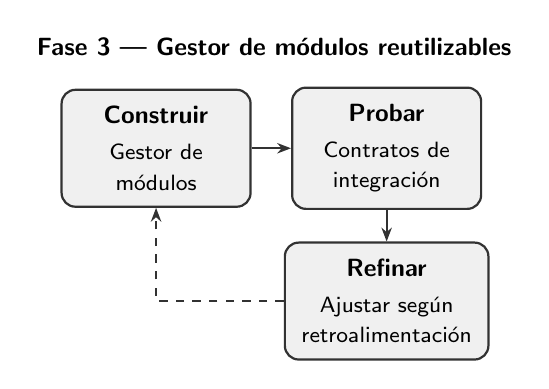
\begin{tikzpicture}[node distance=0.4cm]
    \node[minimum width=16em, minimum height=0pt, inner sep=0pt] (ruler) {};

    \node[font=\sffamily\bfseries\small, align=center,
          below=0pt of ruler] (t3)
      {Fase 3 — Gestor de módulos reutilizables};

    \node[subnode, below=0.3cm of t3, xshift=-1.5cm] (s3a)
      {\textbf{Construir}\\[2pt]
       {\footnotesize Gestor de}\\
       {\footnotesize módulos}};

    \node[subnode, right=0.5cm of s3a] (s3b)
      {\textbf{Probar}\\[2pt]
       {\footnotesize Contratos de}\\
       {\footnotesize integración}};

    \node[subnode, below=0.4cm of s3b] (s3c)
      {\textbf{Refinar}\\[2pt]
       {\footnotesize Ajustar según}\\
       {\footnotesize retroalimentación}};

    \draw[inner arrow, solid] (s3a) -- (s3b);
    \draw[inner arrow] (s3b) -- (s3c);
    \draw[inner dashed] (s3c.west) -| (s3a.south);
  \end{tikzpicture}
};

% FASE 4
\node[solid block, below=of n3] (n4) {
  \textbf{\normalsize Fase 4 — Evaluación y validación}\\[4pt]
  Caso de estudio:\\ Laboratorio Digital del Banco W \\ Tiempo de configuración, incorporación de módulo, inicio de implementación
};

\draw[main arrow] (n1) -- (n2);
\draw[main arrow] (n2) -- (n3);
\draw[main arrow] (n3) -- (n4);

\end{tikzpicture}
